\section{Resultados experimentales}

\subsection{Ordenamiento de Arreglos Unidimensionales}

La Figura~\ref{fig:sorting} muestra la comparación de tiempo de ejecución entre los cuatro algoritmos de ordenamiento analizados: SelectionSort, MergeSort, QuickSort y std::sort. Los tiempos fueron promediados a partir de tres ejecuciones por caso, y convertidos a segundos. También nos muestra el uso de memoria de estos algoritmos.

\begin{figure}[H]
    \centering
    \begin{minipage}[t]{0.5\textwidth}
        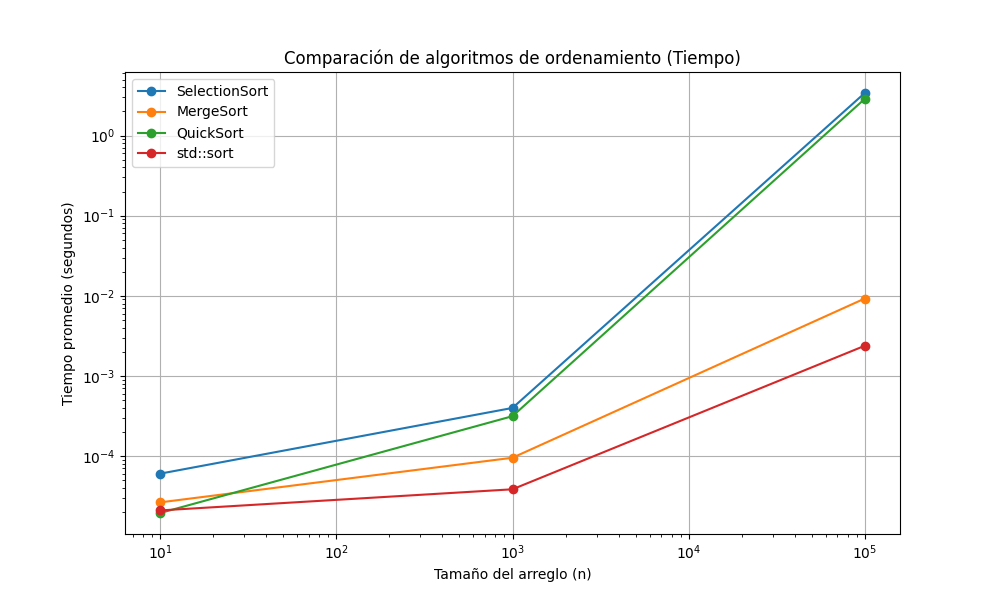
\includegraphics[width=\textwidth]{../code/sorting/data/plots/sorting_comparison_time.png}
    \end{minipage}%
    \begin{minipage}[t]{0.5\textwidth}
        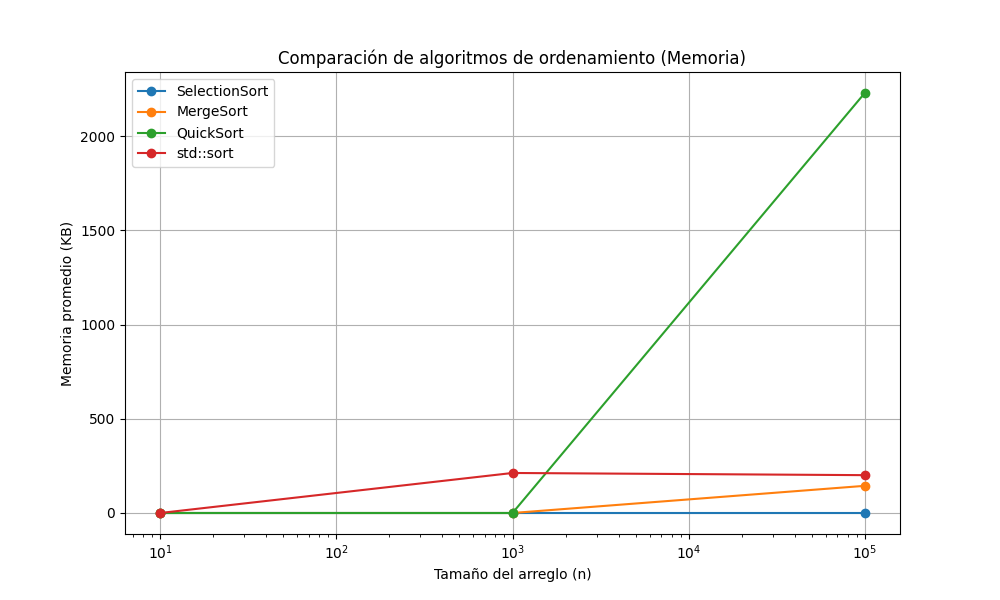
\includegraphics[width=\textwidth]{../code/sorting/data/plots/sorting_comparison_memory.png}
     \end{minipage}%
    \caption{Tiempo de ejecución y uso de memoria de algoritmos de ordenamiento.}
    \label{fig:sorting}
\end{figure}



En términos de tiempo, \texttt{std::sort} demuestra ser el algoritmo más eficiente en todos los tamaños de entrada, seguido por \texttt{MergeSort} y \texttt{QuickSort}, que presentan un comportamiento muy similar. Por otro lado, \texttt{SelectionSort} muestra un rendimiento significativamente inferior, especialmente a partir de $n = 10^3$, reflejando su complejidad cuadrática. Es importante notar que las curvas se ajustan a los comportamientos teóricos esperados, con los algoritmos $O(n\log n)$ creciendo más lentamente que SelectionSort ($O(n^2)$).




En cuanto al uso de memoria, se observa que \texttt{QuickSort} presenta un aumento considerable para $n = 10^5$, lo cual podría deberse a un mal caso de particionamiento o a la implementación que no optimiza la recursión en profundidad. \texttt{std::sort} también presenta un uso mayor comparado con SelectionSort y MergeSort, que se mantienen por debajo de los 200 KB en la mayoría de los casos. En particular, \texttt{SelectionSort} muestra una eficiencia en memoria coherente con su implementación iterativa in-place.

\subsection{Multiplicación de Matrices}

La Figura~\ref{fig:matrix} muestra los resultados obtenidos para la multiplicación de matrices.


\begin{figure}[H]
    \centering
    \begin{minipage}[t]{0.5\textwidth}
        \includegraphics[width=\textwidth]{../code/matrix_multiplication/data/plots/matrix_multiplication_comparison_time.png}
    \end{minipage}%
    \begin{minipage}[t]{0.5\textwidth}
        \includegraphics[width=\textwidth]{../code/matrix_multiplication/data/plots/matrix_multiplication_comparison_memory.png}
     \end{minipage}%
    \caption{Tiempo de ejecución y uso de memoria en la multiplicación de matrices.}
    \label{fig:matrix}
\end{figure}

La Figura~\ref{fig:matrix} muestra el tiempo promedio de ejecución de los algoritmos Naive y Strassen en función del tamaño de la matriz. El algoritmo Naive presenta un mejor desempeño temporal, debido a su bajo overhead computacional. Sin embargo, a partir de tamaños medianos y grandes ($n = 2^8$ y $n = 2^{10}$), se observa que Strassen se logra acercar al método Naive en velocidad, gracias a su menor complejidad asintótican sin embargo esto se podria ver mejor con tamaños mas grandes. ($O(n^{\log_2 7}) \approx O(n^{2.81})$ contra $O(n^3)$).

Los resultados muestran que el algoritmo de Strassen tiene un consumo de memoria considerablemente mayor, especialmente para $n = 1024$, donde supera los 24 MB. Esto se explica por la naturaleza recursiva del algoritmo y la creación repetida de submatrices intermedias. En contraste, el método Naive muestra un crecimiento más moderado y estable, reflejando su simplicidad estructural.

